% CVPR 2027 paper (review). Style files from cvpr-org/author-kit (2026 kit;
% 2027 kit not released at the time of writing). Numbers from
% outputs/reports/OFFICIAL_W_FREEZE.txt. Official Kendall W is never recomputed here.
\documentclass[10pt,twocolumn,letterpaper]{article}

\usepackage[review]{cvpr}

\definecolor{cvprblue}{rgb}{0.21,0.49,0.74}
\usepackage[pagebackref,breaklinks,colorlinks,allcolors=cvprblue]{hyperref}

\def\paperID{*****}
\def\confName{CVPR}
\def\confYear{2027}

\title{Detector Ranking is Not Architecture-Invariant\\under Medical Covariate Shift}

\author{
Anonymous \confName~submission\\
Paper ID \paperID
}

\begin{document}
\maketitle

\begin{abstract}
Post-hoc out-of-distribution (OOD) detectors are almost always ranked on a single backbone.
Holding a medical covariate split fixed, that ranking is not architecture-invariant.
On Camelyon17 hospital-2 (WILDS), Kendall's $W=0.694$ across eight CNN families and seven scores (seed~42).
MSP AUROC spans $0.515$ (ResNet-50) to $0.883$ (DenseNet-121); the DenseNet jump versus the ResNet mean is seed-robust ($0.265{\pm}0.065$, $5/5$ seeds ${\ge}0.15$).
ConvNeXt-Tiny and EfficientNetV2-S@224 hold on $4/5$ seeds, MobileNetV3 and RegNetY on $3/5$; EfficientNet-B3's seed-42 jump is not seed-stable ($2/5$).
Feature-space scores (Mahalanobis, $k$NN) occupy ranks 1--2 on every official backbone.
The same eight-family protocol on skin ISIC$\to$PAD does \emph{not} reproduce the MSP jump ($W=0.791$; Maha rank-1 on $8/8$).
AUROC rank and OOD-triage coverage@risk\,$10\%$ disagree on Camelyon and on MIDOG, and the \emph{sign} of that disagreement flips.
A pre-registered ViT-B/16 Camelyon MSP of $0.884$ met a locked threshold of $0.6947$.
We introduce no new detector:
do not copy an OOD ranking across backbones, and do not pick a backbone for triage from an AUROC table.
\end{abstract}

\section{Introduction}

On the Camelyon17 hospital-2 split, with the same seven post-hoc scores, ResNet-18/50 MSP AUROC is $0.574$/$0.515$ while DenseNet-121 is $0.883$ and EfficientNet-B3 (seed~42) is $0.803$ (Fig.~\ref{fig:msp}).
A practitioner who copies an OpenMIBOOD-style ResNet-50 recipe on this shift and one who uses DenseNet are not looking at the same detector ranking.

That observation is \emph{not} a claim that detector ranking was previously assumed architecture-invariant.
On natural-image \emph{semantic} OOD, ranking already moves with architecture~\cite{zhang2023openoodv15,szyc2023uai,datko2026eswa,claros2025arxiv}.
OpenMIBOOD~\cite{openmibood2025} already showed that ImageNet method ranking does not transfer to medical data and that feature-space scores outperform logit scores under a \emph{frozen} classifier per domain.
Our question is orthogonal: \textbf{holding a medical covariate-shift dataset fixed, how much does detector ranking move when the backbone changes?}

We measure that movement at zoo scale on Camelyon17, show that it does not replicate as an MSP jump on skin ISIC$\to$PAD, and show that AUROC versus operational coverage@risk\,$10\%$ disagrees with a \emph{domain-dependent sign}.
We pre-registered a ViT-B/16 MSP threshold before training that model.
We do not claim a new detector, a Maha${>}$MSP discovery, or a two-domain MSP-jump law.

\paragraph{Contributions.}
\begin{enumerate}
\item \textbf{Camelyon-17, zoo-scale concordance.}
Official Kendall $W=0.694$ ($n{=}8$, 7 methods, seed~42).
The seed-robust MSP jump is DenseNet-121 versus ResNet ($0.265{\pm}0.065$, $5/5$).
ConvNeXt-Tiny and EfficientNetV2-S@224 are $4/5$; MobileNetV3 and RegNetY are $3/5$; EfficientNet-B3 is $2/5$.
Matching the four non-Adam zoo members to ResNet-Adam does not remove those seed-42 jumps.
Feature-space scores stay in the top two ranks.
This is not a claim that architecture-sensitive ranking is new.
\item \textbf{Domain asymmetry.}
Skin ISIC$\to$PAD ($n{=}8$, $W{=}0.791$): Maha rank-1 and $k$NN rank-2 on all eight; MSP stays in a narrow band without a Camelyon-style ResNet-vs-rest jump.
\item \textbf{Utility mismatch is unpredictable.}
Not that AUROC and coverage-based ranking can disagree (AURC/AUGRC already assume that~\cite{geifman2019selectivenet,traub2024augrc}).
The \emph{sign} of AUROC versus coverage@risk\,$10\%$ disagreement flips between Camelyon and MIDOG, with no rule to predict which backbone wins.
\item \textbf{A locked prediction.}
Before training: ViT-B/16 Camelyon MSP ${\ge}0.6947$. Observed $0.884$. Held out of the 8-CNN $W$ on purpose.
\end{enumerate}

\begin{figure*}[t]
\centering
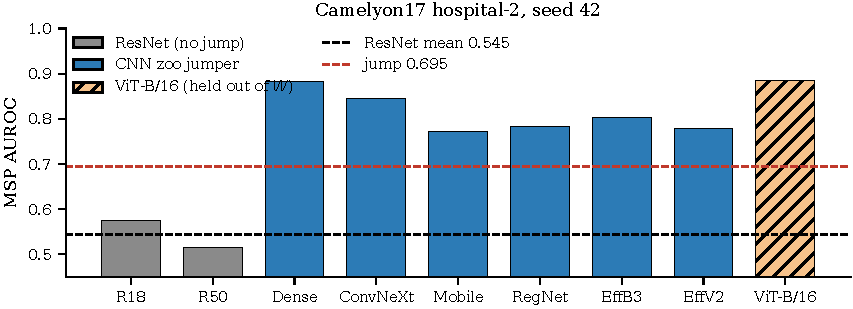
\includegraphics[width=\textwidth]{fig/fig1_msp_bars.pdf}
\caption{\textbf{Camelyon hospital-2 MSP AUROC, seed~42.}
Dashed lines: frozen ResNet mean ($0.545$) and jump threshold ($0.695$).
ViT-B/16 was pre-registered and is not a ninth column of Kendall $W$.
DenseNet, ConvNeXt, MobileNet, RegNet, EffB3, and EffV2-S@224 all clear the bar at this seed; ResNets do not.}
\label{fig:msp}
\end{figure*}

\section{Related work}

OpenMIBOOD~\cite{openmibood2025} ranks 24 post-hoc detectors on three medical benchmarks with a \textbf{single frozen classifier per domain} (ResNet-50 on MIDOG, ResNet-18 on PhaKIR, R(2+1)D on OASIS-3).
It shows that ImageNet method ranking does not transfer to medical data and that feature-space scores outperform logit scores under that fixed-architecture protocol.
It does not measure whether the detector ranking itself is stable across architectures.
We keep their MIDOG split and public ResNet-50 checkpoint as an external reference, and ask the orthogonal question: holding the dataset fixed, how much does detector ranking move when the backbone changes?

OpenOOD v1~\cite{yang2022openood} \emph{fixes architecture on purpose} (LeNet / ResNet-18 / ResNet-50).
That design choice is about v1, not about the later literature.

Architecture-sensitive post-hoc ranking \emph{has} been measured on natural images.
OpenOOD v1.5~\cite{zhang2023openoodv15} evaluates ImageNet-1K post-hoc methods on ResNet-50, ViT-B/16, and Swin-T.
Figure~3 of that paper reports that ``different post-processor may favor different architecture'': ASH/ReAct degrade on transformers, while RMDS suits them.
That study uses three models, semantic near/far OOD, and a qualitative comparison.
It does not compute Kendall's $W$, does not sweep eight CNN families, and is not a covariate hospital shift.
It is the closest natural-image cousin; we do not treat v1.5 as an architecture-fixed protocol.

Szyc \etal~\cite{szyc2023uai} show that detector rankings change across three ResNet-101/110 CIFAR implementation variants with matched closed-set accuracy, and across random seeds, with feature-space methods especially unstable.
That is a reliability result about uncontrolled experimental details on CIFAR semantic OOD, not an eight-family zoo that holds one medical covariate split fixed.
Datko \etal~\cite{datko2026eswa} report a preferred post-hoc detector \emph{per CNN/ViT line}, claimed to be stable across OOD benchmarks for that model---the opposite of a single-split concordance statistic.
Claros Olivares and Brockmeier~\cite{claros2025arxiv} compare a scratch CNN to a fine-tuned ViT and organize confidence-score rankings into cliques by shift severity on CIFAR / TinyImageNet.
Their released results rank scores with AURC/AUGRC; they do not report an AUROC-rank versus coverage@risk\,$10\%$ disagreement whose sign flips across medical covariate domains.

What remains is not the existence of architecture-sensitive ranking.
That existence is published on natural-image semantic OOD.
This paper measures one medical covariate-shift split, held fixed; an eight CNN-family zoo plus a precommitted ViT; Kendall's $W$ per domain; a structured MSP jump whose seed-robust core is DenseNet versus ResNet, with feature methods in ranks 1--2; skin non-replication of the MSP jump; an iWildCam miss on natural-image covariate shift; and the coverage sign-flip below.
iWildCam is the natural-image covariate check we actually ran; OpenOOD v1.5 Fig.~3 is semantic ImageNet, not a substitute.

OoD-Bench~\cite{ye2022oodbench} quantifies OOD \emph{generalization}, not post-hoc detection; we cite it as venue precedent for a two-axis evaluation paper.
WILDS Camelyon17 and iWildCam~\cite{koh2021wilds} supply the hospital / camera-trap covariate splits; iWildCam is a negative bound, not a third main domain.

\section{Setup}

\subsection{Shifts}

Camelyon17 WILDS~\cite{koh2021wilds}: hospitals 0, 3, 4 as ID and hospital~2 as OOD; founding cell, official $W$, $n{=}8$.
Skin ISIC$\to$PAD~\cite{pacheco2020pad}: feature rank-stability without an MSP jump.
MIDOG~\cite{openmibood2025}: OpenMIBOOD 1a vs.\ 1b{+}1c, coverage sign-flip; official $W$ is $n{=}3$.
We build on OpenMIBOOD's public MIDOG split and ResNet-50 checkpoint as an external reference.
Public R50 AUROC ${\sim}0.59$ is \emph{theirs}; in-house R50 MSP $0.512$ is \emph{ours}. We never mix the two.

\subsection{Backbones}

Eight CNN-family models, ImageNet initialization, 10-epoch fine-tune, seed~42, train-frac $1.0$ on Camelyon: ResNet-18/50~\cite{he2016resnet}, DenseNet-121~\cite{huang2017densenet}, ConvNeXt-Tiny~\cite{liu2022convnext}, MobileNetV3-Large~\cite{howard2019mobilenetv3}, RegNetY-3.2GF~\cite{radosavovic2020regnet}, EfficientNet-B3~\cite{tan2019efficientnet} at native 300, and EfficientNetV2-S~\cite{tan2021efficientnetv2} at \textbf{224} (native 384 dropped).
Standard fine-tune recipes (Adam / AdamW / SGD) follow each family's common practice and are \emph{not} forced-identical Adam.
That confound is measured in Sec.~\ref{sec:m1m2}.
Only resolution was isolated in a controlled pair (EffB3 @224 vs.\ @300; EffV2-S @224 vs.\ @384).
ViT-B/16~\cite{dosovitskiy2021vit} @224 is held out of $W$.

\subsection{Scores and statistics}

Seven post-hoc scores: MSP~\cite{hendrycks2017baseline}, Energy~\cite{liu2020energy}, energy of logit-normed logits (ELogitNorm), ViM~\cite{wang2022vim}, ReAct~\cite{sun2021react}, Mahalanobis with Ledoit--Wolf covariance~\cite{lee2018mahalanobis,ledoit2004well}, and $k$NN~\cite{sun2022knn}.
Primary concordance: \textbf{Kendall's $W$ per domain, never pooled}.
Jump: $\mathrm{MSP}-\mathrm{mean}(\mathrm{R18},\mathrm{R50})\ge 0.15$.
Feature drag: Maha or $k$NN on a new backbone below $\mathrm{median}(\mathrm{R18},\mathrm{R50},\mathrm{EffB3})-0.10$.
Official Camelyon ResNet mean MSP ${=}0.544654$; jump iff MSP ${\ge}0.695$ on that split.

Coverage@risk\,$10\%$ is OOD-triage: rank OOD samples by MSP (higher ${=}$ more ID-like) and take the largest coverage whose classifier risk is ${\le}10\%$.
ID-selective Camelyon is vacuous (ID-val acc ${\approx}99.5\%$) and is not cited.

We tested whether the Camelyon MSP pattern is an artifact of input resolution, temperature scaling~\cite{guo2017calibration}, ID-only detector \emph{selection}, a CE{+}SupCon recipe~\cite{khosla2020supcon}, or train-time HED stain jitter.
None is a clean account (Sec.~\ref{sec:failed} and the supplement).

\section{Results}

\subsection{Camelyon-17: official table and five-seed MSP}
\label{sec:camelyon}

Official Kendall $W=\mathbf{0.694}$ ($n{=}8$, 7 methods).
This is the only Camelyon number called ``official $W$.''
Leave-one-backbone recomputation of $W$ ranges $0.676$--$0.738$; that is \emph{structural} sensitivity of the concordance statistic, not a $95\%$ CI (supplement).

\begin{table*}[t]
\centering
\small
\setlength{\tabcolsep}{6pt}
\begin{tabular}{@{}lccccc@{}}
\toprule
Backbone & input & Maha (rank) & $k$NN (rank) & MSP & seed-42 jump \\
\midrule
ResNet-18 & 224 & 0.956 (1) & 0.936 (2) & 0.574 & no \\
ResNet-50 & 224 & 0.896 (1) & 0.866 (2) & 0.515 & no \\
DenseNet-121 & 224 & 0.988 (1) & 0.973 (2) & 0.883 & yes \\
ConvNeXt-Tiny & 224 & 0.928 (1) & 0.916 (2) & 0.846 & yes \\
MobileNetV3-L & 224 & 0.870 (2) & 0.904 (1) & 0.771 & yes \\
RegNetY-3.2GF & 224 & 0.964 (1) & 0.956 (2) & 0.784 & yes \\
EfficientNet-B3 & 300 & 0.885 (2) & 0.934 (1) & 0.803 & yes \\
EfficientNetV2-S & \textbf{224} & 0.880 (1) & 0.856 (2) & 0.778 & yes \\
\bottomrule
\end{tabular}
\caption{Camelyon hospital-2 AUROC, \textbf{seed~42} (official $W$).
Jump iff MSP ${\ge}0.6947$ vs.\ frozen ResNet mean $0.544654$.
MSP range is ResNet-50${\to}$DenseNet.}
\label{tab:cam}
\end{table*}

Feature methods occupy ranks 1--2 on every official backbone (Maha \#1 on $6/8$; $k$NN \#1 on EffB3 and MobileNet).
No backbone drags Maha/$k$NN past the $0.10$ feature-drag threshold.
On Table~\ref{tab:cam}, MSP spans $0.515$--$0.883$; Maha $0.870$--$0.988$; $k$NN $0.856$--$0.973$.
Incomplete concordance ($W{=}0.694$) is the logit ranks moving (Fig.~\ref{fig:ranks}).

\begin{table*}[t]
\centering
\small
\begin{tabular}{@{}lccccccl@{}}
\toprule
Backbone & 42 & 43 & 44 & 45 & 46 & jump mean${\pm}$sd & ${\ge}0.15$ \\
\midrule
ResNet-18 & 0.574 & 0.712 & 0.601 & 0.524 & 0.581 & --- & --- \\
ResNet-50 & 0.515 & 0.621 & 0.619 & 0.515 & 0.661 & --- & --- \\
ResNet mean & 0.545 & 0.667 & 0.610 & 0.520 & 0.621 & --- & --- \\
DenseNet-121 & 0.883 & 0.865 & 0.868 & 0.845 & 0.826 & $0.265{\pm}0.065$ & $5/5$ \\
ConvNeXt-Tiny & 0.846 & 0.799 & 0.803 & 0.764 & 0.785 & $0.207{\pm}0.067$ & $4/5$ \\
MobileNetV3-L & 0.771 & 0.728 & 0.815 & 0.780 & 0.745 & $0.175{\pm}0.081$ & $3/5$ \\
RegNetY-3.2GF & 0.784 & 0.778 & 0.836 & 0.830 & 0.724 & $0.198{\pm}0.089$ & $3/5$ \\
EfficientNet-B3 & 0.803 & 0.731 & 0.643 & 0.818 & 0.678 & $0.142{\pm}0.125$ & $2/5$ \\
EfficientNetV2-S@224 & 0.778 & 0.744 & 0.808 & 0.846 & 0.835 & $0.210{\pm}0.089$ & $4/5$ \\
\bottomrule
\end{tabular}
\caption{Same eight Camelyon hospital-2 MSP cells on all five seeds $\{42,43,44,45,46\}$.
Jump ${=}$ MSP minus that seed's ResNet mean; bar $0.15$.
The last column is how many of those five seeds clear the bar.
Official $W$ is seed~42 only.}
\label{tab:seeds}
\end{table*}

Table~\ref{tab:seeds} reports the full five-seed MSP matrix.
DenseNet-121 is the confirmed seed-robust jump ($5/5$).
ConvNeXt-Tiny and EfficientNetV2-S@224 are not seed-42 flukes ($4/5$); we do not promote them to $5/5$.
MobileNetV3 and RegNetY are $3/5$.
EfficientNet-B3 is $2/5$: its seed-42 jump ($+0.258$) is a favorable draw relative to $0.142{\pm}0.125$.
The seed-42 matrix still shows a jump without feature drag.
The prose claim is narrower than ``$6/6$ non-ResNet, confirmed.''

\subsection{Skin ISIC$\to$PAD is not a second A}

Official $W=\mathbf{0.791}$ ($n{=}8$).
Maha is rank-1 and $k$NN rank-2 on \textbf{all eight} (Fig.~\ref{fig:ranks}).
MSP sits in a narrow band ($0.68$--$0.74$).
There is no Camelyon-style ResNet-vs-rest MSP jump.
EffV2-S@224 MSP is $0.737$; the native-384 cell that put $k$NN at rank~7 (MSP $0.823$) is a resolution artifact and is not in official $W$.
Skin is rank-stability of feature scores under a zoo: a replication of OpenMIBOOD's feature${>}$logit pattern \emph{across architectures}, not an MSP-jump.

\begin{figure*}[t]
\centering
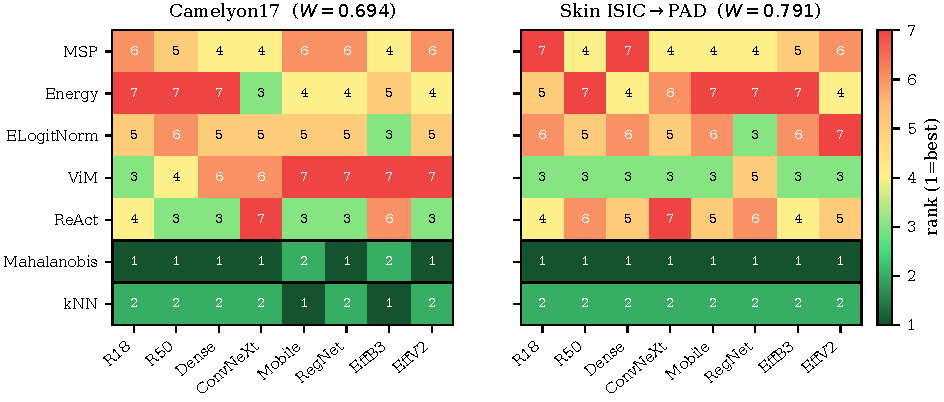
\includegraphics[width=\textwidth]{fig/fig2_rank_heatmaps.pdf}
\caption{\textbf{Method rank by backbone} (1${=}$best AUROC).
Feature-space scores occupy ranks 1--2 on every official backbone in both domains.
Logit ranks move on Camelyon ($W{=}0.694$) and much less on skin ($W{=}0.791$), where Maha is rank-1 on $8/8$.}
\label{fig:ranks}
\end{figure*}

\subsection{Resolution, then optimizer}
\label{sec:m1m2}

Resolution is not the Camelyon DenseNet / seed-42 pattern.
EffB3 Camelyon: $0.803$ @300 ${\to}$ $0.787$ @224 (the jump versus the official ResNet mean survives).
EffV2-S Camelyon: $0.726$ @384 ${\to}$ $\mathbf{0.778}$ @224 (the official cell; the jump is not a 384 artifact).
On skin, the EffV2-S @384 $k$NN collapse \emph{is} a resolution artifact and disappears at 224.
These two facts are not a slogan that ``resolution never matters.''

\paragraph{M1 --- jumpers trained with ResNet Adam}
($\mathrm{lr}{=}10^{-4}$, $\mathrm{wd}{=}10^{-4}$, batch $64$).
The four official zoo members whose standard recipe was not that Adam still jump versus the frozen official ResNet mean $0.545$:
ConvNeXt $0.820$ ($+0.275$), MobileNetV3 $0.737$ ($+0.193$), RegNet $0.805$ ($+0.261$), EffV2-S@224 $0.873$ ($+0.328$); all with id-val acc ${\ge}0.994$.
$4/4$ clean hits.
DenseNet and EffB3 already shared ResNet-Adam in the official zoo.
Recipe mismatch does \emph{not} explain the seed-42 jumps of those four members.
M1 is seed~42 only; the five-seed MSP matrix is Table~\ref{tab:seeds}.

\paragraph{M2 --- ResNets trained with ConvNeXt AdamW}
($\mathrm{wd}{=}0.05$).
ResNet-18 MSP $\mathbf{0.773}$ (enters the $0.695$ band; id-val $0.9957$).
ResNet-50 MSP $0.581$ (stays out; id-val $0.9958$).
ResNet \emph{can} jump under a non-default recipe.
Architecture is not a clean variable, independent of optimizer.
These two results point in opposite directions; we report both.

\subsection{Held-out prediction: ViT-B/16}

Locked \emph{before} training, from the seed-42 zoo rule that non-ResNet-like cells jumped: MSP ${\ge}0.6947$.
Linear depth/parameter/receptive-field predictors are invalid on this $n{=}8$ and are not quoted.
Observed MSP $\mathbf{0.884}$, Maha $0.958$, $k$NN $0.941$.
The prediction holds.
Not a ninth $W$ column.

\subsection{Coverage@risk: the sign flips}

Protocol: OOD-triage coverage@risk\,$10\%$ with MSP, not ID-selective coverage.

On Camelyon hospital-2, the locked $n{=}4$ utility table has MSP AUROC order EffB3@300 ($0.803$) ${>}$ EffB3@224 ($0.787$) ${>}$ ResNet-18 ($0.574$) ${>}$ ResNet-50 ($0.515$), but coverage@risk\,$10\%$ order ResNet-50 ($0.149$) ${>}$ ResNet-18 ($0.145$) ${>}$ EffB3@300 ($0.107$) ${>}$ EffB3@224 ($0.013$).
The AUROC winner is not the coverage winner (Fig.~\ref{fig:cov}).

On MIDOG, official $n{=}3$ (in-house): MSP AUROC ResNet-50 $0.512$, EffB3 $0.486$, ResNet-18 $0.438$ (gaps are small).
Coverage@risk\,$10\%$: EffB3 $0.712$, ResNet-18 $0.442$, ResNet-50 $0.166$.
ResNet-50 is AUROC-highest and coverage-lowest.
The permutation is \emph{not} the Camelyon permutation.

\begin{figure*}[t]
\centering
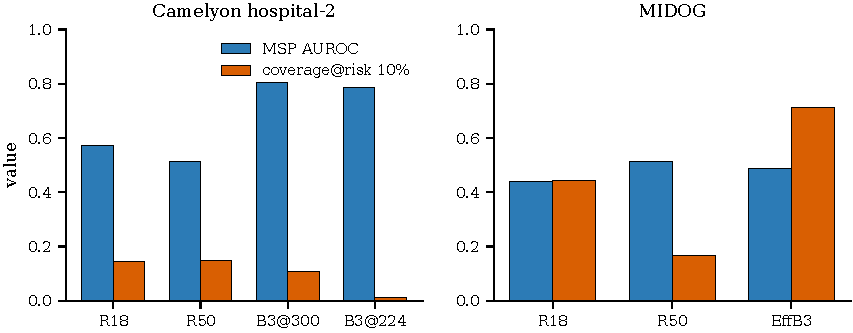
\includegraphics[width=0.92\textwidth]{fig/fig3_coverage_signflip.pdf}
\caption{\textbf{AUROC vs.\ coverage@risk\,$10\%$.}
On Camelyon the AUROC-high EfficientNets have the \emph{lowest} triage coverage; on MIDOG the AUROC-high ResNet-50 is coverage-lowest.
The sign of the disagreement flips.}
\label{fig:cov}
\end{figure*}

We do not write ``AUROC-winner ${=}$ utility-loser'' as a law, and we do not claim to have discovered that AUROC and coverage-based ranking can disagree---AURC/AUGRC exist because that is already assumed.
The increment is narrower: the \emph{sign} of the disagreement flips between two medical covariate-shift domains under the same protocol, with no rule to predict which backbone wins.
Do not choose a backbone for triage from an AUROC leaderboard; measure coverage@risk on the deployment domain.
The Camelyon $n{=}8$ family span still disagrees (DenseNet AUROC $0.883$ / coverage $0.078$; MobileNet coverage $0.904$); that is the same sign-flip claim, not a new official $W$.

\subsection{Frozen foundation models}

We do not claim a foundation-model invert on Camelyon.
Linear-probe MSP: GigaPath~\cite{xu2024gigapath} $0.664$, Phikon~\cite{filiot2023phikon} $0.605$, UNI~\cite{chen2024uni} $0.599$, all ${>}0.5$.
MIDOG UNI / GigaPath MSP $0.445$ / $0.470$ in a sign audit is a MIDOG-only footnote, not a Camelyon invert.
FM Maha ${\sim}0.995$--$1.0$ is discussion support that feature${>}$logit can survive a training-paradigm change, under the ranking-stability question, not a pillar.

\section{Failed alternatives}
\label{sec:failed}

Each of the following was a precommitted test. None is hidden.

\textbf{Resolution} (from Sec.~\ref{sec:m1m2}).
EffB3@224 MSP $0.787$; EffV2-S@224 MSP $0.778$.
Not a pixel-size explanation of Table~\ref{tab:cam}.

\textbf{Temperature $T^\ast$.}
Correlation of $T^\ast$ with the MSP jump: $r{=}0.268$, $p{=}0.52$.
DenseNet${-}$ResNet-18 MSP gap $0.308{\to}0.308$ after $T^\ast$.
Calibration/temperature is not the mechanism.
We do not write a monotonicity theorem relating temperature scaling to MSP AUROC.

\textbf{ID-only Maha/MSP gate.}
Selecting a score from ID-only statistics is a \emph{selector}, not a detector.
On Camelyon it picks Maha on $2/8$ backbones; mean AUROC of the gated score $0.837$ versus always-Maha $0.940$.
The bar was matching Maha and ViM. It does not.

\textbf{CE{+}SupCon} ($\lambda{=}0.1$, $\tau{=}0.07$), ResNet-18 ${+}$ DenseNet.
Gap $0.308{\to}0.238$ ($23\%$; precommit bar was $50\%$ / ${\le}0.154$).
ResNet-18 MSP $0.574{\to}\mathbf{0.515}$ (worse; this is the SupCon cell, not official ResNet-50 MSP $0.515$).
Part of the shrink is the low model degrading.
Dirty; not a recipe.

HED stain jitter, an in-house MIDOG $n{=}8$ zoo, and a shift-type extract (covariate / task / far-OOD) are in the supplement.
Joint readout: no shift-type law, no stain mitigation, no Camelyon-style MSP jump on MIDOG.
We do not open center-loss, triplet, a coverage surrogate, or an ensemble.

\section{Discussion and limitations}

Under this histopathology hospital shift, logit OOD scores move with the backbone: seed-robust for DenseNet ($5/5$), present on most seeds for ConvNeXt and EffV2-S@224 ($4/5$), weaker for MobileNet and RegNet ($3/5$), and seed-fragile for EfficientNet-B3 ($2/5$).
Feature-space scores are the stable default \emph{when the shift looks like Camelyon}.
That is a protocol warning, not a new detector.

On skin, feature rank-stability holds \emph{without} an MSP jump.
Architecture-instability of MSP is not a cross-medical law.
OpenMIBOOD's feature${>}$logit finding is replicated here under a zoo; the increment is ranking movement, when it happens, plus the operational AUROC${\leftrightarrow}$coverage mismatch.
ViT-B/16 was a locked prediction, not a post-hoc ninth CNN.
M1 and M2 disagree about how cleanly that movement is ``architecture'' versus optimizer; both stand.

\paragraph{Limitations.}
(1)~\textbf{iWildCam bound.}
Locked 3-backbone cell: DenseNet MSP $0.575$ vs.\ ResNet mean $0.604$, jump $-0.029$.
Extra five CNNs vs.\ that domain's ResNet mean: ConvNeXt $0.601$, MobileNet $0.558$, RegNet $0.580$, EffB3 $0.577$, EffV2-S $0.650$; $0/5$ jump.
We do not see the Camelyon MSP-jump on this non-medical covariate shift.
The phenomenon may be biomedical-specific.
We did not hunt a fourth medical domain and do not pool iWildCam with Camelyon $W$.
(2)~\textbf{No clean mitigation.}
CE{+}SupCon is dirty (ResNet-18 MSP worse).
HED stain jitter is dirty (DenseNet MSP $0.780{<}0.80$ precommit floor).
The ID-only gate is a selector.
(3)~\textbf{MIDOG official $W$ is $n{=}3$} (in-house R18/R50/EffB3, $W{=}0.857$).
An in-house $n{=}8$ zoo shows no MSP jump and does not replace official $W$.
(4)~$W$ is per-domain; do not average $0.694$ / $0.791$ / $0.857$.
(5)~No reader study: the operational claim stops at coverage@risk.
(6)~Architecture is confounded with its standard training recipe.
$5/5$ seed-robustness is DenseNet only.
Official $W$ stays seed~42.
We did not isolate staining vs.\ scanner vs.\ tissue prep inside the hospital shift.

We will release the architecture-zoo evaluation and coverage@risk code, crediting OpenMIBOOD for MIDOG imglists, the public ResNet-50 checkpoint, and the 1a / cs-ID / near-OOD protocol.

\section{Conclusion}

Under Camelyon hospital shift, post-hoc detector choice is backbone-dependent: a seed-robust DenseNet MSP jump, weaker but directionally present jumps on ConvNeXt/EffV2 ($4/5$) and MobileNet/RegNet ($3/5$), and a seed-fragile EfficientNet-B3 cell.
Feature-space ranks stay in the top two whether that jump is present (Camelyon) or absent (skin).
A pre-registered ViT hit shows the Camelyon logit instability is not only a CNN-zoo accident; it did not appear on iWildCam.
AUROC and coverage@risk can rank backbones in opposite orders, and which way the disagreement points depends on the domain.
There is no new method in this paper.
The result is the protocol: do not copy an OOD ranking across backbones, and do not pick a backbone for triage from an AUROC table.

{\small
\bibliographystyle{ieeenat_fullname}
\bibliography{refs}
}

\end{document}
